%%!TEX root = dissertation.tex
\setcounter{chapter}{2}
\chapter{The structure of acoustic voice variation in bilingual speech}
\label{ch3:Voice}


% add a structure in variability section so i can cite the face stuff in the intro

\section{Introduction}\label{ch3:sec:introduction}
Voices provide a lot about the person talking, ranging from their current physical and emotional state to talker indexical features that help listeners identify who they are. In this context, voices can be described as auditory faces, in that they are uniquely individual, yet with broadly shared characteristics across the population \citep{belin_2004_voice}. Voices are rich in information, and they convey all of this information alongside communicative content. Understanding the structure of a voice is no small feat, as is understanding how listeners use different dimensions within the voice in processing talker indexical, affective, social, and linguistic information. The difficulty here arises from the sheer variability across voices. While voices share attributes and relevant acoustic dimensions, much of the variation appears idiosyncratic \citep{lee_2019_acoustic}. From the perspective of voice perception, the balance between shared and idiosyncratic makes sense. The shared dimensions allow listeners to perceive, classify, and understand new voices, while the idiosyncrasies enable identification and discrimination between voices. While this makes sense conceptually, understanding the structure of voice variation in speech production and its complement in listeners' ability to process that information remains an active area of research. While the focus of this chapter is acoustic voice variability, the emphasis on describing and processing variation echoes one of the largest puzzles in phonetics: the ``lack of invariance'' problem \citep{liberman_perception_1967}. That is, given the ubiquity of variation, how do perceivers efficiently extract relevant and important information from the communicative signal? 

While variation is indeed wide-ranging, it remains far from random. Some of the most prevalent accounts of how individuals understand and process variation emphasize that variation in speech production is highly structured. This chapter looks at the structure of voices, and the following chapter examines structure for sound categories---both attempt to elucidate what exists in the signal for listeners to use.  In the domain of voice quality, Jody Kreiman and colleagues have synthesized work from various areas and put forth a psychoacoustic model of voice quality \citep{kreiman_2014_theory}. This model features a minimal set of acoustic dimensions necessary to encode (and thus reproduce) voice quality. While there are numerous dimensions in the model, extensive experimental work has validated the inclusion of each dimension \citep[][and references therein]{kreiman_2021_validating}. As a result, Kreiman and colleagues argue that this set is both sufficient and necessary to capture a wide range of normal and disordered voices. This model includes acoustic dimensions that capture harmonic and inharmonic voice source, pitch, loudness, and vocal tract characteristics. While each dimension in the model could be considered independently by researchers, Kreiman and colleagues argue that these dimensions are more than the sum of their parts. The measures covary and conspire together to form a percept. While this model establishes a set of acoustic dimensions, it does not arbitrate between them in a way that establishes what matters for a given voice in a given language. 

There is a large body of literature focused on understanding differences in variability across populations for a small set of acoustic measurements. Such studies typically compare summary statistics for fundamental frequency (F0) and a handful of spectral measures. This body of work will be summarized below in the context of crosslinguistic comparisons. Before summarizing this work, it is important to highlight that very little of it dives into the structure of voice variability, which is a relatively new area spearhead by Lee and colleagues \citep{lee_2019_acoustic, lee_2019_spontaneous, lee_2020_language}. In this set of studies examining acoustic voice variation in different languages and speech styles, the authors leverage the psychoacoustic model of voice quality \citep{kreiman_2014_theory} and adapt methods from the domain of face variability and perception \citep{burton_2016_faces}. The driving question for Lee and colleagues is one of understanding what information exists in the signal and how it's structured. In many ways, this is the first step towards understanding which aspects of voice are available to listeners and thus useable in perceptual processes. 

%%Intro clean up to here

\citet{lee_2019_acoustic} find... \hl{Flesh out description of paper here}. The same group of authors replicated this finding in connected speech \citep{lee_2019_spontaneous} and in Seoul Korean \citep{lee_2020_language}, with relatively minor differences that have straightforward explanations. 


Across these three studies, Lee and colleagues argue for a prototype model of voice perception based on production data regarding how individuals deviate from a speech community average (i.e., the prototypical voice). These results largely mirror findings from the face variability domain.

The prototype model argument is perhaps easier to conceptualize with faces. \citet{burton_2016_faces} find that faces share a set of relevant dimensions in how they vary. These are things like ..., that is ar eyou looking at a face straight on? In profile? Another shared dimension is lighting. These are things that all faces are subject to. idiosyncratic dimensions are things like expressions, makeup, or facial hair. There might be broad similarity across different subsets of individuals, but not all faces vary over time in that way. The analogs for voice are somewhat less readily available, but nonetheless relevant. \citet{lee_2019_acoustic}\hl{ find that....}

Despite the high degree of variability, idiosyncrasies, and similarity or deviation from a prototype, listeners nonetheless use talker-specific information to recognize and discriminate voices. Listeners are good at identifying familiar voices, but perform poorly on the same tasks with unfamiliar voices \citep{nygaard_1998_talker}. It was suggested by \citet{lee_2019_acoustic} that familiarity with a voice largely comes from learning how that voice varies across time and space, whether within an utterance or across environments, physical states, and emotions.
\hl{evidence here from talker identification and discrimination work that there si both linguistic and crosslinguistic type stuff}

\citet{lee_2019_acoustic} restrict variability in their analysis by focusing on English speech produced by native English speakers from the UCLA Variability Speaker Database \citep{keating_2019_database}. \hl{They use....methods.}

This work is groundbreaking in a lot of ways, even if it looks only at a particular dialect and register of American English spoken by monolinguals in southern California \hl{CHECK}. It is comforting that subsequent work by Lee and colleagues has extended the basic conceptualization to connected speech \citep{lee_2019_spontaneous} and to Seoul Korean \citep{lee_2020_language}. Across the original paper and follow up presentations, voice variability was largely accounted for by harmonic and noise spectral shape parameters associated with a voice's timbre (brightness, breathiness). In the extension to English connected speech, the behavior of fundamental frequency differed, with it accounting for more variation in spontaneous speech. This tracks from assumptions about read speech following more predictable (monotone) patterns, and spontaneous speech being more affective in nature. In the case of Seoul Korean sentence reading, fundamental frequency and lower formant frequencies emerged as important dimensions of variation. The authors argue that this reflects phrasal intonation patterns that occur in reading. 

While this body of work compares outcomes for English speakers and Korean speakers, the groups considered are necessarily distinct populations. \citet{lee_2020_language} argue that there are both language and biologial factors contribute to the structure of voice variation. Bilingual speech would be an ideal testing ground for examining this distinction. The (likely unintended) dichotomy of language and biology is misleading. While there are ultimately vocal tract and other biological constraints on a voice, individuals show remarkable control over the space \citep{}, and are capable of manipulating factors that are not linguistically important but which signal social and contextual information. This applies both within languages \citep{}, as well as across languages in the case of bilinguals \citep{bullock_2009_sociophonetics}. Thus in the case of bilinguals, the only aspect we can be truly confident in being held constant across languages is the biological part. The same hardware can be used for drastically differnt ends. 

In this chapter, I examine how voice varies across a bilingual's two languages. Some differences are expected. Languages differ in terms of their consonant and vowel inventories, which affect the spectral properties of a language. While all languages have consonants and vowels, they differ with respect to distribution, articulation, and acoustics \citeeg{munson_2010_deconstructing}. \hl{For example...phrasal accent stuff in korean, danish vowels vs. 3-vowel system, slavic consonants vs hawaiian} 


Some prior work has looked at various vocal features across languages, both in the case of bilinguals and comparing separate monolingual populations. While this work uses rather broad strokes to compare crosslinguistic behavior---things like means and standard deviations, as opposed to a deep dive into the structure of variability---it captures some interesting and useful generalizations, suggesting that while some aspects of voice variability differ for linguistic reasons, other talker-indexical features remain constant across languages, and still others can be influenced by both linguistic and non-linguistic factors. 

Suprasegmental and prosodic properties also vary across languages. Languages can differ in terms of whether a suprasegmental dimension is exploited at all---for example, does a language encode lexical tone contrastively? Another way language vary in this respect is in how they carve up the suprasegmental space. For example, how many lexical tones are there? What shapes of tone are present? \hl{Expand this}

Within an individual bilingual, the acoustic variability within each language can also be related to the social identities a talker adopts within each language (see discussion in \citet{cheng_2020_f0}). Further, bilinguals are sophisticated social actors, and can conciously leverage their use of language to convey different aspects of identity\hl{... add more here}

In an effort to understand what aspects of an individual's voice vary across languages and what are more or less fixed talker-specific attributes, researchers have compared particular spectral properties of bilingual speech, both within and across talkers. Results have been decidedly mixed \citep{cheng_2020_f0,altenberg_2006_f0,ryabov_2016_self}. \hl{Big picture summary, and flesh out each of the following in greater detail.}

For example, a small group of English-Cantonese bilinguals (n$=$9) in did not differ in mean fundamental frequency (F0), but exhibited greater variability in F0 \citep{altenberg_2006_f0}. 

This was not the case in \citet{ng_2012_ltas}, which examined voice differences with Cantonese-English bilinguals reading passages (n = 40). Based on Long-Term Average Spectral measures, females exhibited higher F0 in English than Cantonese, but males did not \citep{ng_2012_ltas}. In the same study, all participants had greater mean spectral energy values (mean amplitude of energy between 0--8 kHz) and lower spectral tilt (ratio of energy between 0--1 kHz and 1--5 kHz) in Cantonese \citep{ng_2012_ltas}. Respectively, these findings suggest a greater degree of laryngeal tension and breathier voice quality in Cantonese compared to English.

While the body of work in this area on Cantonese-English bilinguals remains small, there are useful insights from other similar language pairs. \hl{In a study of Mandarin and English...}

Not all factors are necessarily easy to separate as linguistic or talker-instrinsic. For example... \hl{Speech rate shared across languages, for example}

% NOT SURE WHERE TO PUT THIS CHUNK %%
That bilingual listeners are sensitive to this information signals its importance \citep{orena_2019_identifying,fricke_2016_phonetic}. The following paragraphs summarize this work.
\hl{Talker identification generalizes, but not amazingly well} % work on this during writing time friday
%%%%%%%%%%%%%%%%%%%%%%%%%%%%%%%%%%%%


Together, these bodies of literature raise the question of whether bilingual talkers have the ``same'' voice in each of their languages. Using the corpus described in Chapter \ref{ch:Corpus}, I look at spectral properties \citep{cheng_2020_f0,altenberg_2006_f0, ryabov_2016_self,ng_2012_ltas}, and also examine how acoustic variation is structured, following the work of \citet{kreiman_2014_theory} and \citet{lee_2019_acoustic}. \hl{Describe and discuss psychoacoustic voice quality model}

This work builds on \citet{lee_2019_acoustic} in a handful of ways: it extends the methods to the case of bilinguals, considers longer samples, and addresses the role of sample duration both within and across talkers and languages. 

\section{Methods \& Results}\label{ch3:sec:methods_results}
\subsection{Data}\label{ch3:sec:data}
The data used in this analysis come from the conversational interviews in the SpiCE corpus---both Cantonese and English are considered. As noted before, the 34 talkers studied here are all early Cantonese-English bilinguals. For additional information about the participant, please refer to sections \ref{ch2:subsec:participants} and \ref{ch2:sec:statistics} in the previous chapter. 

While prior work uses short chunks of speech, the present analysis is focused on longer stretches of spontaneous speech. Additionally, there are practical reasons to exclude the sentence reading and storyboard tasks from this analysis. \hl{The sentence sets...} Similarly, there are imbalances in the storyboard task. As talkers narrated the same story in both languages, they were often more confident the second time around. 

%The 34 talkers studied here come from the SpiCE corpus of bilingual speech in Cantonese and English \citep{johnson_2020_spice}. The corpus comprises two conversational interviews with early bilinguals---one in each language. While these interviews were conducted in either Cantonese or English, code-switching occurred regularly within each interview. Talkers were of a similar age (\textit{Mdn} = 21, \textit{M} = 22.4, \textit{SD} = 4), learned both languages from an early age (Cantonese: \textit{Mdn} = 0, \textit{M} = 0.03, \textit{SD} = 0.2; English: \textit{Mdn} = 0, \textit{M} = 1.32, \textit{SD} = 1.8), and considered themselves to be proficient speakers (Cantonese: Good/Excellent = 29, Fair = 5; English: Good/Excellent = 33; Fair = 1). Talkers, however, had varied language background profiles (e.g., locations lived, dialects, knowledge of other languages), and should not be characterized as a homogeneous bilingual group. This heterogeneity is an accurate representation of the Cantonese speech community \citep{liang_2015_china} and it is considered a boon in this study, as analyses are conducted on a within-talker basis. 

% The audio recordings are high quality, with a 44.1 kHz sampling rate, 24-bit resolution, and minimal background noise. Both the participant and interviewer wore head-mounted microphones connected to separate channels, and levels were adjusted to minimize speech from the other talker. 

As discussed in the previous chapter, the recordings are high-quality, with a 44.1 kHz sampling rate, 16-bit resolution, and minimal background noise. As a reminder, both the participant and interviewer wore head-mounted microphones connected to separate channels, and levels were adjusted to minimize speech from the other talker. For the analysis in this chapter, the participant channel was extracted from the stereo recordings, including any code-switches they made during the interview. While it would be possible to exclude items not produced in the main interview language from the final sample using the time-aligned transcripts, this was not done. The driving reason for keeping code-switches in the analysis is that such code-switches are representative of the particular talker's language behavior. Further, just because someone switches lanuages, does not mean that they full switch. For example, individual words may be borrowed in and pronounced with the phonology of the main language. 
% SHOULD I go back and re-do this for just the same-as-interview-language chunks? 

All voiced segments were identified with the \textit{Point Process (periodic, cc)} and \textit{To TextGrid (vuv)} Praat algorithms \citep{boersma_2021_praat}, implemented with the Parselmouth Python package \citep{jadoul_2018_parselmouth}. The pitch range settings used with \textit{Point Process (periodic, cc)} were set to 100--500 Hz for female talkers, and to 75--300 for male talkers. While speech from the interviewer can occasionally be heard in the participant channel, it is quiet enough to have been largely ignored by the Praat algorithms. This method of identifying voiced portions of the speech signal captures vowels, approximants, and some voiced obstruents. This differs slightly from the methods described in \citet{lee_2019_acoustic}, the paper on which the methods of this chapter were modeled. 

\subsection{Acoustic measurements}\label{ch3:sec:acoustic}
All voiced segments were subjected to the same set of acoustic measurements of voice quality made by \citet{lee_2019_acoustic}, with the exception of formant dispersion, which was excluded given its near perfect correlation with the measured value of F4. The choice of measurements in \citet{lee_2019_acoustic} comes from the psychoacoustic voice quality model described in the introduction to this chapter \citep{kreiman_2014_theory}. Measurements were made every 5 ms during voiced segments, as in \citet{lee_2019_acoustic}, using VoiceSauce \citep{shue_2011_voicesauce}.  measurements were: 

\begin{description}
    \item[F0] Fundamental frequency is a correlate of pitch and is associated with linguistic (e.g., lexical tone), prosodic, and talker characteristics. F0 was measured in Hertz using the \hl{ALGORTHIM} \citep{}, which is widely regarded to be more accurate that the alternative choices in VoiceSauce. It is one of the more widely studied variables on this list, as evidenced by the literature cited in the introduction \citep[e.g.,][]{}
    \item[F1, F2, and F3] The first three formant frequencies---also measured in Hertz---are typically discussed in relation to linguistic contrasts, particuarly  vowel and sonorant consonants. 
    \item[F4] The fourth formant frequency is not typically discussed in linguistic contexts, and is instead associated with talker characteristics. In this light, it is not particularly surpriseing that it was highly correlated with formant dispersion. Both measures reflect talker characteristics such as vocal tract length. F4 is measured in Hertz.
    \item[H1*--H2*] The corrected amplitude difference between the first two harmonics is one of four primary measures used to characterize source spectral shape \citep{kreiman_2014_theory}. It is associated with phonation type, \hl{and blah blah blah}. The asterisks here and in the following spectral slope measures indicated that the value has been corrected \citep{iseli_2007_voice}, in order to account for \hl{the impact of nearby formants on the amplitudes of harmonics.}  \hl{units} 
    \item[H2*--H4*] The corrected amplitude difference between the second and fourth harmonics is the second of four measures capturing spectral shape. \hl{It is associated with...}  \hl{units}
    \item[H4*--H2kHz*] The corrected amplitude difference between the fourth harmonic and the harmonic closest to 2000 Hz is the third spectral shape measure. Unlike the previous two, one of the harmonics depends of F0, while the other does not. It captures shape in a higher frequency range, \hl{and is typically associated with...}  \hl{units}
    \item[H2kHz*--H5kHz*] The corrected amplitude difference between the harmonics closest to 2000 Hz and 5000 Hz is a measure of harmonic spectral slope that does not depend on. It captures the highest frequency band of the four shape measures, \hl{and it is associated with...}  \hl{units}
    \item[CPP] Cepstral Peak Prominence is a measure of the ratio between harmonic energy and spectral noise, and is associated with non-modal phonation types. As CPP is a ratio, it does not have units.
    \item[Energy] Root Mean Square (RMS) \textbf{Energy} is a measure of spectral noise that reflects overall amplitude. \hl{units}
    \item[SHR] The subharmonics-harmonics amplitude ratio is a measure of spectral noise associated with period doubling or irregularities in phonation. While based on amplitude, this ratio is unitless. 
\end{description}

\hl{The raw data output from VoiceSauce is available in the supplementary materials for this dissertations.} % decide how, but probably data>OSF and code>GitHub

\subsection{Exclusionary criteria and post-processing}

Given the nature of the corpus and methods thus far, there is reason to suspect a sizable number of erroneous measurements. In an effort to filter these out prior to analysis, measurements were subjected to exclusionary criteria focused on identifying impossible values. Observations were excluded in cases where any of the following measurements had a value of zero: F0, F1, F2, F3, F4, CPP, or (uncorrected) H2kHz--H5kHz. Filtering based on F0 and the four formant frequencies reflects the observation that zero measurements are not possible for voiced portions of the speech signal. \hl{Filtering with CPP says...} Only one of the uncorrected harmonic amplitude measures, as erroneous values tended to co-occur on the same observation, and the distribution of H2kHz--H5kHz did not span zero, with the exception of a spike of (erroneous) values equal to zero. This operationalization minimizes the removal of correctly measured zero values, which would have occurred with one of the other spectral shape parameters (corrected or uncorrected). 

Moving standard deviations were calculated for each of the 12 measures using a centered 50 ms window, such that each window includes approximately ten observations. The moving standard deviations capture dynamic changes for each of the voice quality measures, which is important as they may better reflect what listeners attend to in talker identification and discrimination tasks \citep{lee_2019_acoustic}. This analysis uses moving standard deviations, as opposed to the coefficients of variation used by \citet{lee_2019_acoustic}. This should not have any undue effect on the outcome, as all variables were scaled prior to inclusion in the principal components analysis described in the next section. The last round of exclusionary criteria uses these moving standard deviations. If an observation was missing a moving standard deviation value, it was removed. This means that obsevations falling extremely close to a voicing boundary were not included. 

Overall, there were 24 total measures, with a measured value and a moving standard deviation for each of the acoustic measurements listed above. These 24 measures are used in the analyses described in the following sections. Across the 34 talkers, there were 3,126,267 observations after winnowing the data. These observations were not evenly distributed across talkers and langauges. \hl{NEW not implemented yet:} In order to control for the impact of passage length in the analysis, the number of samples for each talker was capped to include only the first 22,433 samples were considered for each interview. This value was selected as it represents the interview with the fewest number of samples across all talkers and languages. Following this last winnowing step, there were 1,525,444 total observations. While the winnowing process removed a lot of data, the number of samples here is still substantially larger than used in \citet{lee_2019_acoustic}, where the per-talker sample count was closer to 5,000. Further, a later section in this chapter directly tackles the issue of passage length, and (spoiler) indicates that 20,000 is sufficient for stabilization.

\subsection{Crosslinguistic comparison of acoustic measurements} %% need to re-do the numbers in this section or decide not to

Following from prior work, the first step in this analysis is a crosslinguistic comparison for each talker and measure. As discussed in the introduction to this chapter, there are some often (but not always) found differences for Cantonese and English. \hl{ADD 1-SENTENCE SUMMARY}

Figure XX depicts the distribution of values for each of the measurments across languages. Given the highly skewed shape of 


For each acoustic measurement and talker, I conducted a Student's \textit{t}-test and calculated Cohen's \textit{d}, in order to give a high-level assessment of whether variable means differed across the two languages. These comparisons have no bearing on how a given variable \textit{varies}. Table~\ref{ch3:tab:cohend} reports counts of talkers by effect size. Notably, across all talkers and variables, only 21.1\% yielded non-trivial Cohen's \textit{d} values. Most talkers (32/34) had at least one non-trivial comparison. The distribution of these counts is depicted in Figure~\ref{ch3:fig:ntcounts}. 

\begin{table}[htbp]
\caption{This table reports counts of Cohen's \textit{d} for crosslinguistic comparisons of each of the acoustic measurements by talker. Degrees of freedom ranged between 49,274--136,644 across t-tests. For most talkers and variables, the difference in means was trivial, which is reflected in that column's high counts.}
\label{ch3:tab:cohend}
\centering
\begin{tabular}{lccc}
\toprule
         & \multicolumn{3}{c}{\textbf{Cohen's \textit{d}}} \\
         & \textbf{Trivial} & \textbf{Small} & \textbf{Medium} \\
\textbf{Variable} & \textbf{\textit{0.0--0.2}} & \textbf{\textit{0.2--0.5}} & \textbf{\textit{0.5--0.8}} \\ 
\midrule
F0 & 21 & 10 & 3 \\
F0 s.d. & 34 & 0 & 0 \\
F1 & 24 & 9 & 1 \\
F1 s.d. & 29 & 5 & 0 \\
F2 & 26 & 8 & 0 \\
F2 s.d. & 32 & 2 & 0 \\
F3 & 24 & 9 & 1 \\
F3 s.d. & 29 & 5 & 0 \\
F4 & 30 & 3 & 1 \\
F4 s.d. & 28 & 6 & 0 \\
H1*--H2* & 18 & 15 & 1 \\
H1*--H2* s.d. & 32 & 2 & 0 \\
H2*--H4* & 25 & 9 & 0 \\
H2*--H4* s.d. & 31 & 3 & 0 \\
H4*--2kHz* & 25 & 8 & 1 \\
H4*--2kHz* s.d. & 34 & 0 & 0 \\
H2kHz*--5kHz* & 23 & 10 & 1 \\
H2kHz*--5kHz* s.d. & 31 & 3 & 0 \\
CPP & 21 & 10 & 3 \\
CPP s.d. & 32 & 2 & 0 \\
Energy & 17 & 14 & 3 \\
Energy s.d. & 18 & 16 & 0 \\
SHR & 31 & 3 & 0 \\
SHR s.d. & 29 & 5 & 0 \\
\bottomrule
\end{tabular}
\end{table}

\begin{figure}[htbp]
\begin{center}
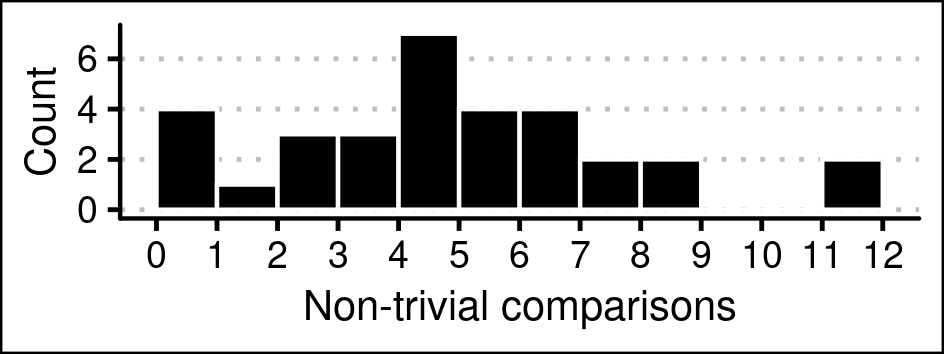
\includegraphics[width=0.875\linewidth]{figures/3-non-trivial_counts_by_talker.png} 
\caption{A summary of the number of non-trivial comparisons from Table~\ref{ch3:tab:cohend} across the 34 talkers.}
\label{ch3:fig:ntcounts}
\end{center}
\end{figure}

For the non-trivial comparisons, there were consistent patterns across languages for H1*--H2* and F0. For the remaining variables, while some talkers exhibited a difference in mean values, the direction of the difference varied, or relatively few talkers exhibited the difference. 

H1*--H2* was significantly higher in Cantonese for a relatively large subset of the talkers (13/34), lower for a small number (3/34), but trivial for most (18/34). While based on a different measure than \citep{ng_2012_ltas}, this is consistent with the finding that Cantonese tends to be breathier, or English creakier---the current analysis does not distinguish between these interpretations.

If there was a non-trivial difference in F0 across languages, then Cantonese had a lower mean F0 than English (13/34; Female = 7), though most talkers did not exhibit a difference (21/34). This is consistent with prior findings that when a difference between English and Cantonese was found, Cantonese had a lower mean F0 for females \citep{ng_2012_ltas,altenberg_2006_f0}. I also observe this difference for a small number of males. 


\subsection{Principal components analysis}\label{ch3:sec:pca}
\subsubsection{Methods}
Principal components analysis (PCA) is a dimensionality reduction technique appropriate for data that include a large number of (potentially) correlated variables. The distillation into components helps identify and facilitate describing the internal structure, in this case, of a voice. While the typical goal in analyses that use PCA is to identify a smaller number of components to use in modeling, the focus here is instead on understanding the internal structure. In this light, the components themselves will be examined.

I adapt methods from work on voices \citep{lee_2019_acoustic,lee_2020_language} and faces \citep{burton_2016_faces,turk_1991_eigenfaces}. The goal is to the capture similarities or differences in the structure of each talker's voice across languages. As such, I conducted PCAs separately for each talker-language pair, and compared the results of each talker's English and Cantonese PCAs. All 24 measures were normalized (z-scored) on by-PCA basis prior to the analysis. PCAs were implemented with the \textit{parameters} package \citep{makowski_2019_parameters} in R \citep{r_2021}, using an oblique \textit{promax} rotation to simplify the factor structure, as the measurements reported in the previous section were expected to be somewhat correlated given prior findings \citep{lee_2019_acoustic}, and a broader undesttanding of how different acoustic measures align with one another \citep{kreiman_2014_theory, kreiman_2021_validating}.

Each PCA included the number of components for which all resulting eigenvalues were greater than 0.7 times the mean eigenvalue, following Jolliffe's \citep{jolliffe_2002_pca} recommended adjustment to the Kaiser-Guttman rule. I used this rule, rather than a more sophisticated test (e.g., broken sticks), as it is not detrimental to our exploratory analysis to err on the side of including marginal components. Additionally, across each of the components, only loadings with an absolute value of 0.32 or higher were interpreted \citep{lee_2019_acoustic,tabachnick_2013_statistics}.

\subsection{PCA results}\label{ch3:sec:pca_results} 
The PCAs across both languages for all 34 talkers resulted in 10--15 components and accounted for 74.6--85.8\% of the total variation. A slight majority of talkers had the same number of components for each of their languages (18/34). Of the remainder, most talkers had a difference of one in the number components (14/34), and far fewer differed by two (2/34). Table XX details the number of components and variance accounted for across all talkers and languages. 

\hl{TABLE HERE}

To assess whether talkers exhibit the same structure in voice variability across their languages, I first consider the patterns present across the different PCAs, as this provides context for understating what unique structural characteristics in talkers' voices looks like. To this end, I briefly summarize common patterns across PCA components, regardless of how much variance they account for, as the difference is often quite small. Figure~\ref{ch3:fig:VF32A} shows the first four components of a single talker's Cantonese and English PCAs, illustrating some examples of how components can vary (or not) across languages. It also highlights the importance of not attributing to much value to the ordering of components, but rather to their composition and variance accounted for.

\begin{figure}[htbp]
\begin{center}
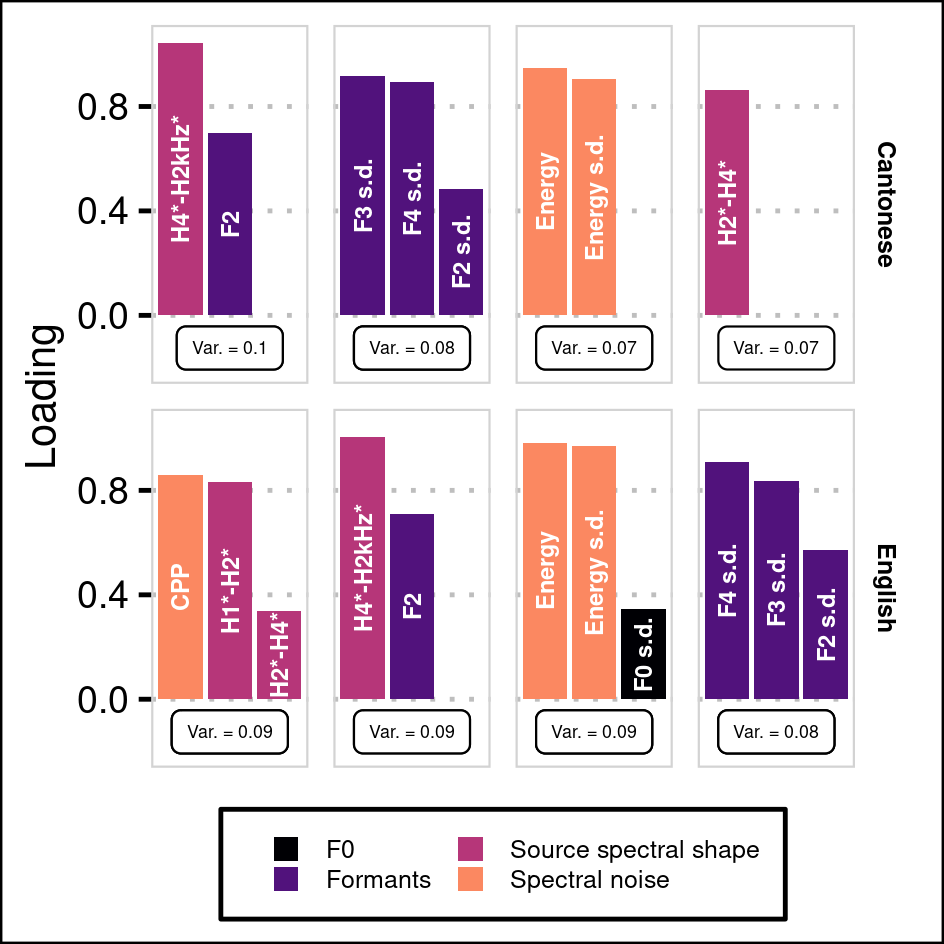
\includegraphics[width=0.875\linewidth]{figures/3-VF32A_pretty.png} 
\caption{In the first four components of a talker's Cantonese and English PCAs, loadings are represented by bar height and are labelled with the variable name; color represents conceptual groupings; and, the component's variance is superimposed.}
\label{ch3:fig:VF32A}
\end{center}
\end{figure}

Broadly speaking, there were a lot of similarities in component composition across both talkers and languages, with the eight most commonly occurring components summarized in Table~\ref{ch3:tab:components}. For context, recall that PCAs had anywhere from 10--15 components total. These eight components consisted of source spectral shape, spectral noise, as well as formant variables. On the other hand, F0 co-occurred with a wide variety of variables (often Energy), but in a manner that was less consistent across talkers. There were additional components (not reported here) that were shared by less than half of talkers. In summary, despite the greater amount of shared structure across PCAs than found in \citet{lee_2019_acoustic}, there is still ample room for idiosyncratic variation, both in terms of which variables co-occur, as well as in how much variance different components account for. 

\begin{table}[th]
\caption{A summary of the most commonly occurring components across all PCAs. Variables are only included if $|$Loading$|>$ 0.32. Italics indicate additional variables that were present on a component for a subset of talkers (i.e., an alternative but related configuration). \textit{N} indicates the number of times a component occurred (out of 34), and \textit{Var. \%} gives the range of percent variance accounted for by the component.}
\label{ch3:tab:components}
\centering
\begin{tabular}{lcccc}
\toprule
 & \multicolumn{2}{c}{\textbf{Cantonese}} & \multicolumn{2}{c}{\textbf{English}} \\
\textbf{Variables} & \textbf{N}  & \textbf{Var. \%}  & \textbf{N}  & \textbf{Var. \%} \\
\midrule
\begin{tabular}[c]{@{}l@{}}H4*--H2kHz*,\\ H2kHz*--H5kHz*, F2, \\\textit{F3}, \textit{F4}\end{tabular} & 34 & 9.3--15.5 & 32 & 9.2--16.7 \\
\midrule
\begin{tabular}[c]{@{}l@{}}H4*--H2kHz* s.d.,\\ H2kHz*--H5kHz* s.d.\end{tabular} & 32 & 6.3--8.3  & 34 & 4.1--5.0  \\
\midrule
\begin{tabular}[c]{@{}l@{}}Energy, Energy s.d, \textit{F0}\end{tabular} & 31 & 5.8--9.4  & 33 & 6.3--9.1  \\
\midrule
CPP s.d. & 29 & 4.1--5.0  & 31 & 4.1--4.9  \\
\midrule
\begin{tabular}[c]{@{}l@{}}SHR, SHR s.d.\end{tabular} & 30 & 3.8--7.5  & 29 & 5.4--7.3  \\
\midrule
\begin{tabular}[c]{@{}l@{}}F3, F4, \textit{F2}\end{tabular} & 26 & 6.0--8.5  & 29 & 5.8--8.5  \\
\midrule
\begin{tabular}[c]{@{}l@{}}F3 s.d., F4 s.d., \textit{F2 s.d.}\end{tabular} & 26 & 5.3--8.6  & 29 & 4.7--8.6  \\
\midrule
\begin{tabular}[c]{@{}l@{}}H2*--H4* s.d., \\H1*--H2* s.d.\end{tabular} & 26 & 4.2--6.5  & 28 & 4.2--6.8  \\
\bottomrule
\end{tabular}
\end{table}


\subsection{Canonical redundancy analysis}
\subsubsection{Methods}
In order to assess whether variation in a talker's voice is structurally similar across both languages, I compare PCA output from both languages by calculating redundancy indices in a canonical correlation analysis \citep[CCA][]{stewart_1968_canonical, jolliffe_2002_pca}.  CCA is a statistical method used to explore how groups of variables are related to one another. The two sets of variables are transformed such that the correlation between the rotated versions is maximized. This is useful here, as a talker may have similar components in their English PCA and Cantonese PCA, but these components might not necessarily be in the same order, even if they account for comparable amounts of variance.

Redundancy is a relatively simple way to characterize the relationship between the loadings matrices of two PCAs---the two sets of variables under consideration here. For example, the two indices represent the amount of variation in a talker's Cantonese PCA output that can be accounted for via canonical variates by their English PCA output, and vice versa. Notably, the two redundancy indices are not symmetrical \citep{stewart_1968_canonical}. This is particularly relevant in cases where the PCAs comprise different numbers of components, as determined by the stopping rule described above.

I computed redundancy indices for all pairwise combinations, including cases where similar values were expected (same talker, different language), and cases where I expected dissimilarity (different talker and language). Considering that the PCA analyses retain the lower-dimensional structure within each language, these redundancy indices effectively reflect the degree to which the lower-dimensional structure of the voice variability is retained across a talker's two languages.

\subsubsection{Results}


Redundancy indices for within-talker comparisons ranged from 0.82 to 0.99, (\textit{Mdn} = 0.93, \textit{M} = 0.92, \textit{SD} = 0.04), and are displayed in Figure~\ref{ch3:fig:redundancy}, with the two redundancy indices for a given pair plotted against one another. Comparisons across talkers within-language (range: 0.63--0.98, \textit{Mdn} = 0.84, \textit{M} = 0.84, \textit{SD} = 0.6) and across-language (range: 0.66--0.98, \textit{Mdn} = 0.83, \textit{M} = 0.84, \textit{SD} = 0.6) are generally lower, but still relatively high. Within-talker values were confirmed to be higher than across-talker comparisons [\textit{Welch's t}(71.36) = --17.83, \textit{p} $<$ 0.001, d = 1.76]. 

The high values are not unexpected. As PCA is a dimensionality reduction technique, the discarded components almost certainly contain idiosyncratic variation. Moreover, and following from Section~\ref{ch3:sec:pca_results}, there were a substantial number of commonly occurring patterns across talkers and languages. 

\begin{figure}[htbp]
\begin{center}
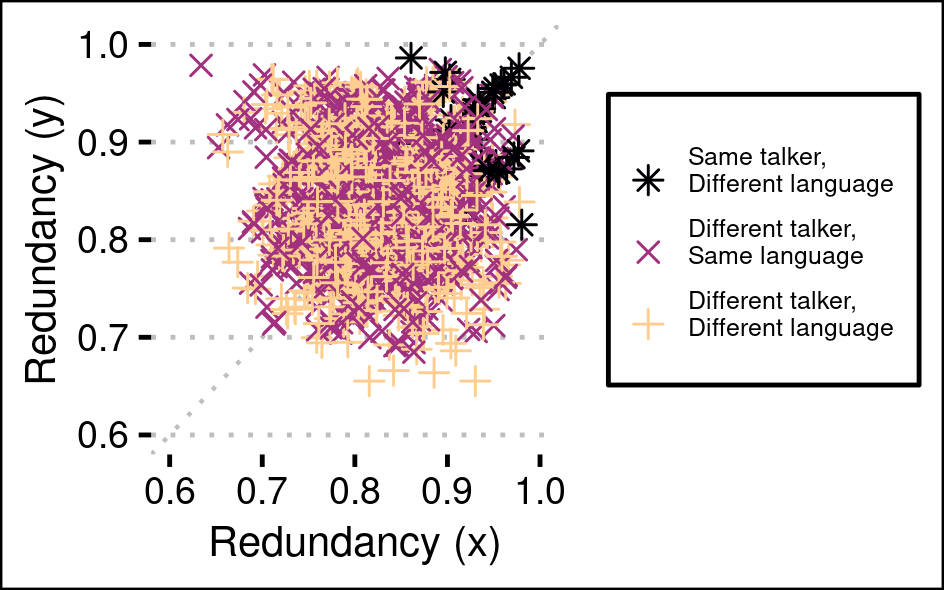
\includegraphics[width=0.875\linewidth]{figures/3-reds_pretty.png} 
\caption{The relationship between the two redundancy indices for three different types of comparisons. Within-talker comparisons are clustered at the top right.}
\label{ch3:fig:redundancy}
\end{center}
\end{figure}






\section{Discussion and conclusion}\label{ch3:sec:discussion}

This study examines spectral properties and structural similarities in an individual's voice in two languages. A clear result is that most of the bilinguals studied here exhibit similar spectral properties, and similar lower-dimensional structure in voice variation, despite substantial segmental and suprasegmental differences across English and Cantonese \citep{matthews_2013_cantonese}. In this sense, a majority appear to have the same ``voice'' across languages, which renders voice-as-an-auditory-face an apt comparison.

The comparison of these 34 Cantonese-English bilinguals' voices across languages suggest more similarity for an individual across languages than found within a more tightly controlled group of monolingual English speakers \citep{lee_2019_acoustic}---several analysis decisions may have contributed to this. I compared similar components independent of order, which ignores the fact that similar components may account for different amounts of variance, but ensures that any comparisons made are among like items. Any downside to this methodological decision is mitigated by the fact that most components made relatively small contributions, accounting for 4.2--10.3\% (95\% highest density interval) of the PCA's total variance. 

While statistical choices may have affected these results, the data differences between the current and previous studies are also important to note. This study uses substantially longer passages than the short samples in \citet{lee_2019_acoustic}. The larger speech sample may allow for a more stable underlying structure to showcase itself, as opposed to the potential for ephemeral variation in a shorter sample. This possibility is easily testable by manipulating the length of the speech sample in the analysis.

Ultimately, the goal is to understand how the acoustic variability and structure of talkers' voices maps onto listeners' organization of a voice space for use in talker recognition and discrimination. Turning to listener and behavioural data will help in deciphering what is meaningful variation within a voice from low level noise that cannot be attributed to a particular vocal signature. Verification from listener performance will help adjudicate which statistical choices present an acoustic voice space that matches listener organization. 

\endinput % -------------------------------------------------------- %
